\chapter{BDD partie 2}


\section{Niveau logique : modèle relationnel}
\subsection{Principe}
On adapte un MCD en tables à deux dimensions.\\
On décide du type des attributs.\\
Pour l'instant, on peut utiliser des types génériques, qui sont susceptibles de varier légèrement d'un SGBD à un autre :
\begin{itemize}
	\item	\mintinline{sql}{INTEGER} pour les entiers;
	\item	\mintinline{sql}{FLOAT} ou \mintinline{sql}{REAL} pour les nombres en virgule flottante;
	\item	\mintinline{sql}{VARCHAR(taille)} ou \mintinline{sql}{TEXT} pour les chaînes de caractères de taille fixe ou illimitée;
	\item 	\mintinline{sql}{BIT} pour les booléens;
	\item 	\mintinline{sql}{DATE} et \mintinline{sql}{TIME} pour les heures et les dates;
\end{itemize}



\subsection{Transformer une entité en relation}
On va transformer chaque entité du MCD en \textit{relation} :
\begin{center}
	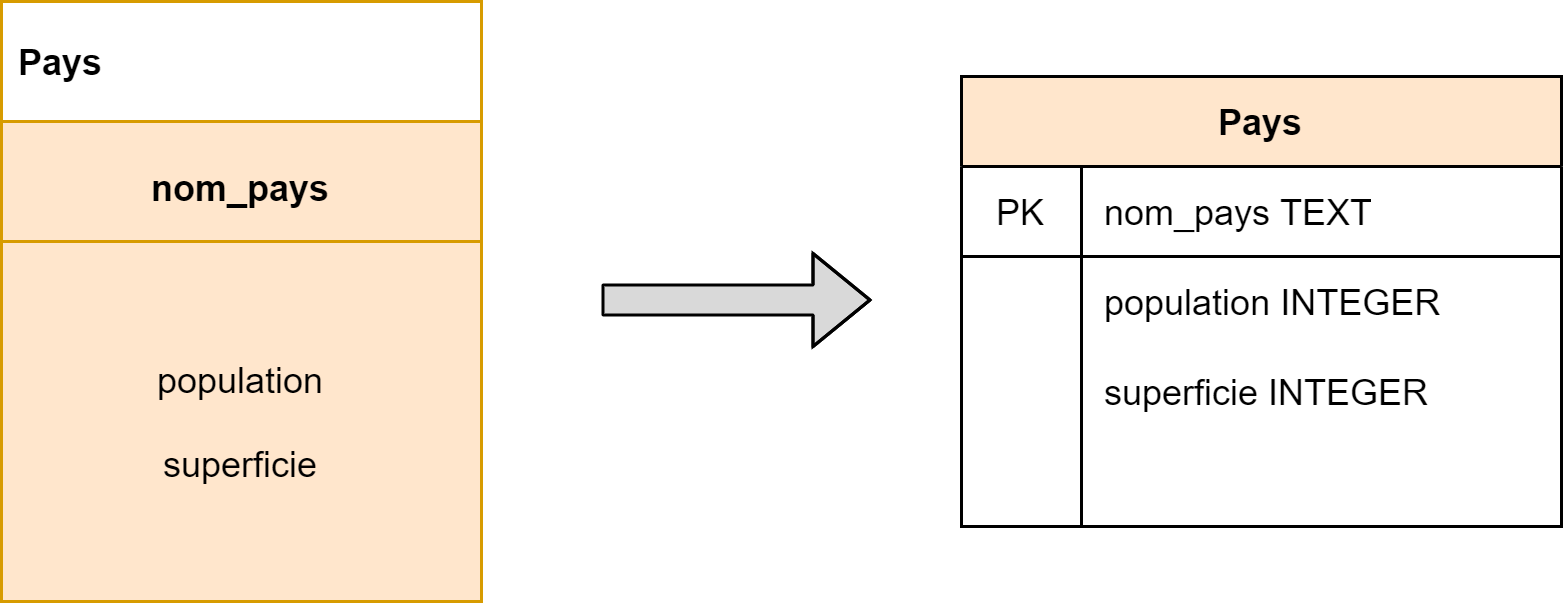
\includegraphics[width=7cm]{img/entite_vers_relation}
\end{center}
On indique les types de chaque attribut de la relation.

Le ou les identifiants de l'entité sont appelés des \textit{clés primaires} pour la relation : « PK» est l'abréviation de \mintinline{sql}{PRIMARY KEY}.\\
Le nom de la relation est noté en gras, la clé primaire soulignée.\\

\textbf{Pays}(\uline{nom\_pays TEXT}, population INTEGER, superficie INTEGER)\\




\subsection{Transformer une association en relation : cas (0,1) ou (1,1)}
\textit{Quand la relation possède une cardinalité valant (0,1) ou (1,1)}
\begin{center}
	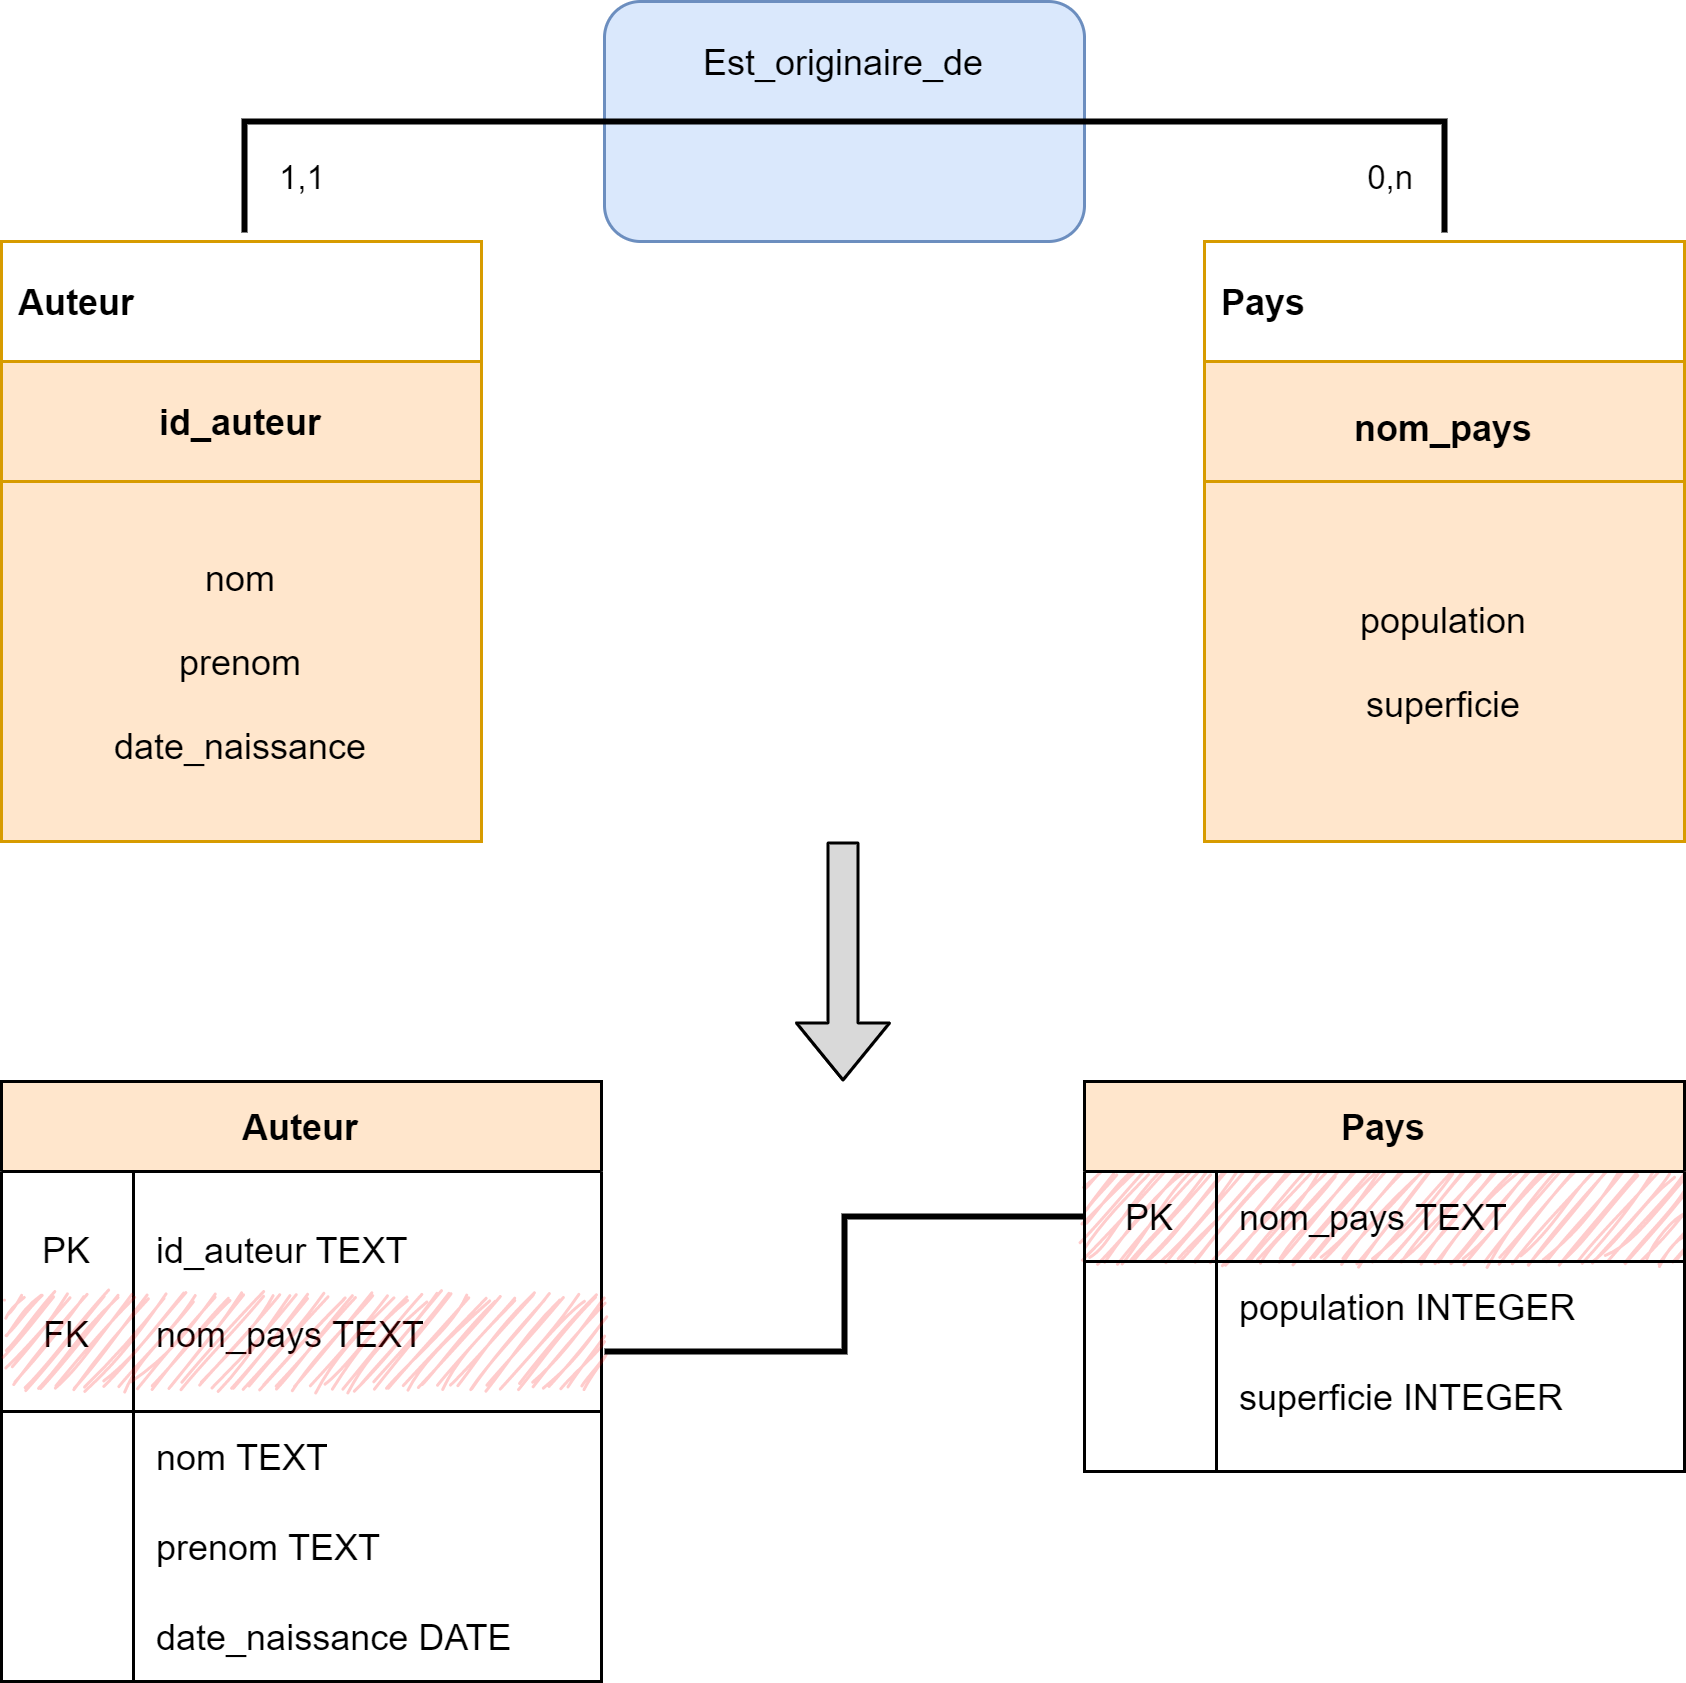
\includegraphics[width=7cm]{img/association_vers_relation_1}
\end{center}




\subsection{Transformer une association en relation : cas (0,1) ou (1,1)}

Puisqu'un auteur vient d'un pays et un seul, on ajoute un attribut nom\_pays à la relation \textbf{Auteur}.

On précise que cet attribut est \textit{nécessairement} l'un des attributs nom de la relation \textbf{Pays} en ajoutant « FK»  dans le tableau , qui est l'abréviation de \mintinline{sql}{FOREIGN KEY}.

On dit que nom\_pays est une \textit{clé étrangère}, qui \textit{fait référence} à l'attribut nom de la relation \textbf{Pays}.

La clé étrangère est soulignée en traits discontinus.\\



\textbf{Pays}(\uline{nom\_pays TEXT }, population INTEGER, superficie INTEGER)\\

\textbf{Auteur}(\uline{id\_auteur INTEGER}, \dashuline{nom\_pays TEXT} , nom TEXT, prenom TEXTE, date\_naissance DATE)


\subsection{Transformer une association en relation : autre cas}
\textit{Quand la relation ne possède pas de cardinalité valant (0,1) ou (1,1)}
\begin{center}
	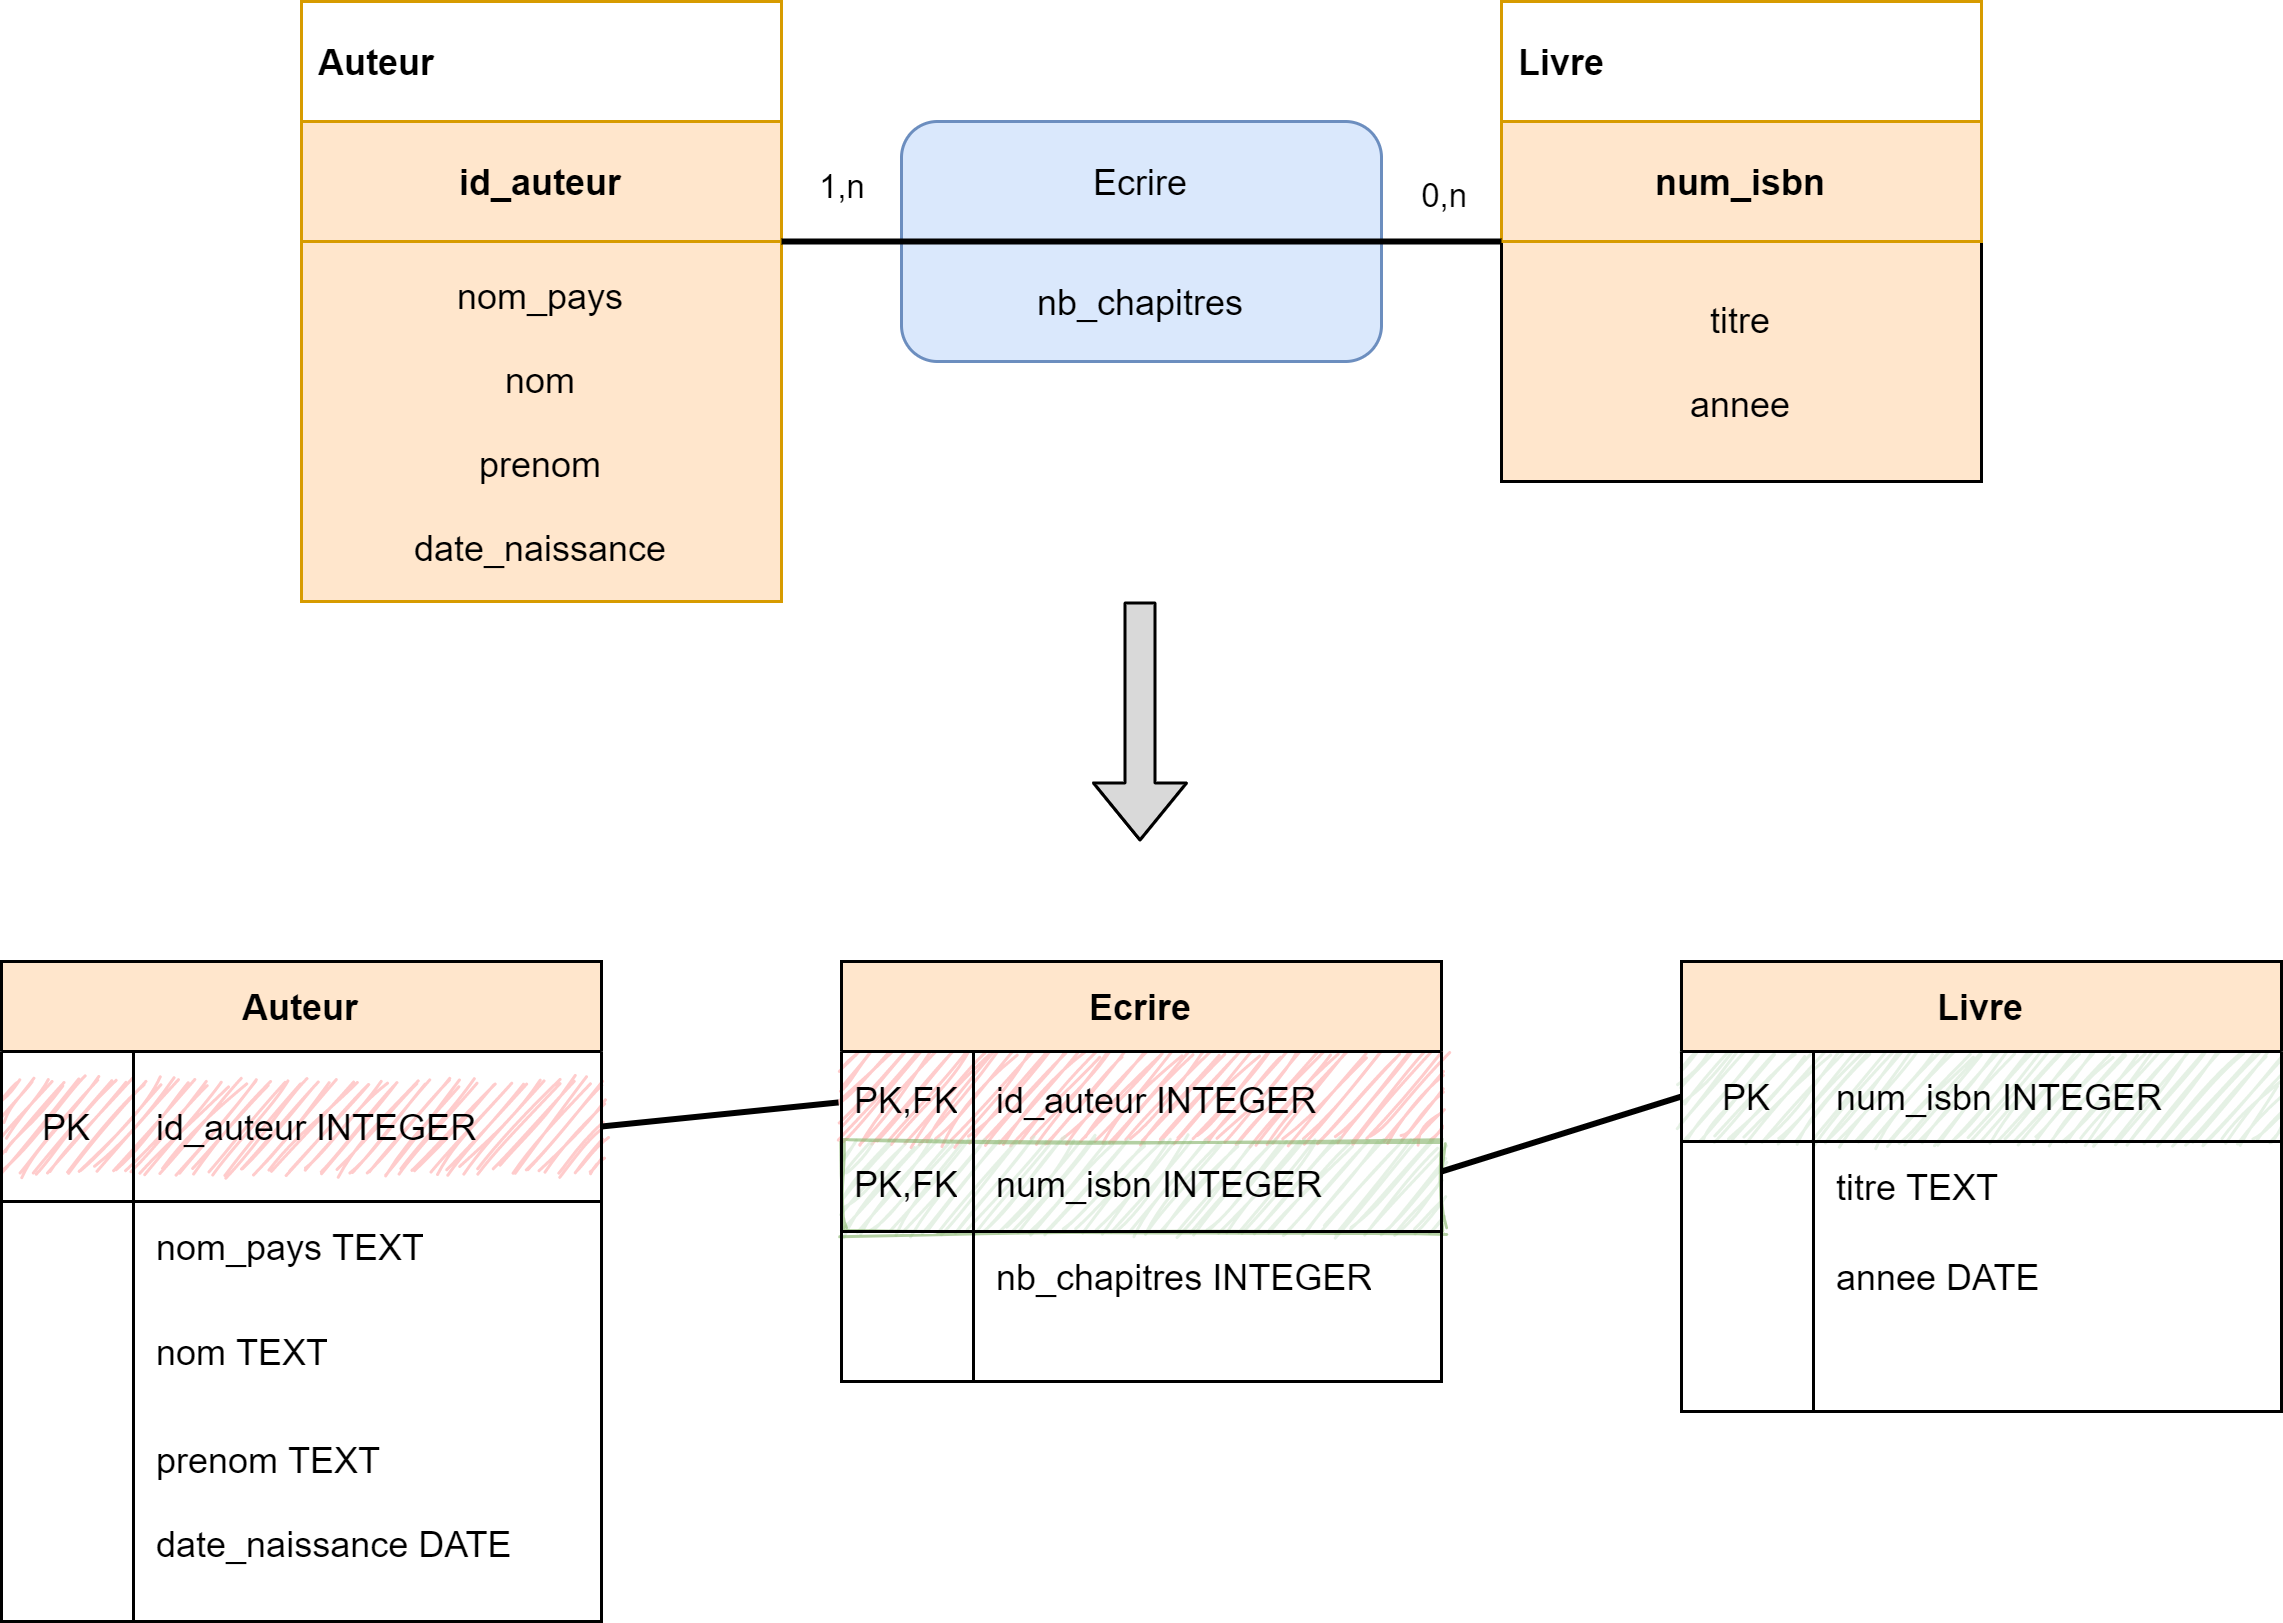
\includegraphics[width=8cm]{img/association_vers_relation_2}
\end{center}


\subsection{Transformer une association en relation : autre cas}
Dans ce cas on fabrique une nouvelle relation :
\begin{itemize}
	\item on considère les clés primaires des relations issues des entités concernées par l'association;
	\item on fabrique une \textit{nouvelle relation} avec comme clé primaire ce couple de de clés primaires;
	\item ces clés primaires sont également des \textit{clés étrangères};
	\item on ajoute si besoin est d'autres attributs spécifiques à l'association.
\end{itemize}
On va noter celaans ce cas on fabrique une nouvelle relation :
\begin{itemize}
	\item on considère les clés primaires des relations issues des entités concernées par l'association;
	\item on fabrique une \textit{nouvelle relation} avec comme clé primaire ce couple de de clés primaires;
	\item ces clés primaires sont également des \textit{clés étrangères};
	\item on ajoute si besoin est d'autres attributs spécifiques à l'association.
\end{itemize}
On va noter cela\\

\textbf{Ecrire}(\uline{\dashuline{id\_auteur INTEGER, num\_isbn INTEGER}}, nb\_chapitres INTEGER)\\

\subsection{Modèle complet}


\textbf{Pays}(\uline{nom\_pays TEXT }, population INTEGER, superficie INTEGER)\\

\textbf{Livre}(\uline{num\_isbn INTEGER} , titre TEXT, annee DATE)\\

{\scriptsize\textbf{Auteur}(\uline{id\_auteur INTEGER}, \dashuline{nom\_pays TEXT} , nom TEXT, prenom TEXTE, date\_naissance DATE)\\}

\textbf{Ecrire}(\uline{\dashuline{ id\_auteur INTEGER, num\_isbn INTEGER}}, nb\_chapitres INTEGER)\\


\begin{remarque}[]
	Lorsqu'on modélise une BDD, on n'a pas toujours besoin de passer par le MCD pour établir le modèle relationnel : on peut parfois le faire directement.
\end{remarque}

\begin{encadrecolore}{Bilan}{UGLiBlue}
	Lorsqu'on établit un modèle relationnel (à partir d'un MCD ou directement) on définit des relations qui symbolisent des entités ou des associations.
	
	On définit aussi les \textit{contraintes} de la BDD :
	\begin{itemize}
		\item	\textit{Contraintes de domaines} : c'est essentiellement définir le type des attributs des relations;
		\item	\textit{Contraintes d'entité} : c'est déterminer des clés primaires pour garantir l'unicité de chaque élément d'une relation;
		\item 	\textit{Contraintes de référence} : c'est déterminer les clés étrangères dans les relations;
		\item 	\textit{Contraintes utilisateur} : ce sont des contraintes sur les valeurs des attributs qui garantissent leur cohérence.
	\end{itemize}
\end{encadrecolore}

\subsection{Contraintes}
Ces contraintes vont garantir la cohérence logique de la future base de données
\begin{itemize}
	\item	à tout instant;
	\item	dans le cas d'une mise à jour des données (insertion ou suppression d'éléments de la relation).
\end{itemize}

\begin{exemple}[ de contraintes utilisateur]
	Dans la relation \textbf{Pays}(\uline{nom\_pays TEXT }, population INTEGER, superficie INTEGER)\\
	
	On peut rajouter les contraintes utilisateurs suivantes :
	\begin{itemize}
		\item 	population > 0;
		\item 	superficie > 0.
	\end{itemize}
	De même dans \textbf{Auteur} et \textbf{Livre} on peut décider que les dates doivent être postérieures à une date donnée.	
\end{exemple}
\section{Exercices}

\begin{exercice}[]
	Reprendre le MCD de l'exercice 3 du chapitre « BBD partie 1» (\textbf{Hotel Reservation Client Chambre}) et donner le modèle relationnel
	\begin{itemize}
		\item	sous la forme d'un schéma;
		\item	sous forme écrite
	\end{itemize}
\end{exercice}

\begin{exercice}[]
	Reprendre le MCD de l'exercice 4 du chapitre « BBD partie 1» (\textbf{Consultation Patient Medicament Medecin}) et donner le modèle relationnel
	\begin{itemize}
		\item	sous la forme d'un schéma;
		\item	sous forme écrite
	\end{itemize}
\end{exercice}

\begin{exercice}[]
	Donner la modélisation relationnelle d'un bulletin scolaire. Elle doit permettre de représenter
	\begin{enumerate}
		\item 	des élèves possédants un numéro d'identifiant alphanumérique unique;
		\item 	des matières, qui grâce à la dernière réforme du lycée, varient d'un élève à l'autre;
		\item 	au plus une note sur 20 par matière.
	\end{enumerate}
\end{exercice}

\begin{exercice}[]
	On modélise un annuaire téléphonique de la manière suivante :\\
	
	\texttt{\textbf{Annuaire}(nom TEXT, prenom TEXT, \uline{tel TEXT})}\\
	
	Dire si les ensembles suivants sont valides pour cette modélisation.
	\begin{enumerate}
		\item 	\texttt{\{\}}
		\item 	\texttt{\{('titi', 'toto', '0123456789')\}}
		\item 	\texttt{\{('titi', 'toto', '0123456789'),('tata', 'tutu', '0123456789')\}}
		\item 	\texttt{\{('titi', 'toto', '0123456789'),('titi', 'toto', '9876543210')\}}
		\item 	\texttt{\{('titi', 'toto', '0123456789'),('tata', 'tutu')\}}
		\item 	\texttt{\{('titi', 'toto', 0123456789)\}}
	\end{enumerate}
\end{exercice}

\begin{exercice}[]
	\begin{enumerate}
		\item 	Proposer une modélisation des départements français. On veut pourvoir stocker le nom, le code, le chef-lieu et la liste de tous les départements voisins.\\
		      Attention les codes de départements ne sont pas tous des nombres : 2A et 2B pour la Corse et les départements d'Outre-Mer ont un code à 3 chiffres.\\
		\item 	Proposer une contrainte utilisateur supplémentaire, non indiquée dans le schéma, pour éviter la redondance d'informations dans la liste des voisins.
	\end{enumerate}
\end{exercice}

\begin{exercice}[]
	Proposer une modélisation du réseau de bus d'une agglomération. Elle doit permettre de générer la liste des horaires passage de chaque bus de chaque ligne pour chaque jour de la semaine arrêt par arrêt.
\end{exercice}
